%% Преамбула TeX-файла

% 1. Стиль и язык
\documentclass[utf8x, 14pt]{G7-32} % Стиль (по умолчанию будет 14pt)

% Остальные стандартные настройки убраны в preamble.inc.tex.
\sloppy

% Настройки стиля ГОСТ 7-32
% Для начала определяем, хотим мы или нет, чтобы рисунки и таблицы нумеровались в пределах раздела, или нам нужна сквозная нумерация.
\EqInChapter % формулы будут нумероваться в пределах раздела
\TableInChapter % таблицы будут нумероваться в пределах раздела
\PicInChapter % рисунки будут нумероваться в пределах раздела

% Добавляем гипертекстовое оглавление в PDF
\usepackage[
bookmarks=true, colorlinks=true, unicode=true,
urlcolor=black,linkcolor=black, anchorcolor=black,
citecolor=black, menucolor=black, filecolor=black,
]{hyperref}

\AfterHyperrefFix

\usepackage{microtype}% полезный пакет для микротипографии, увы под xelatex мало чего умеет, но под pdflatex хорошо улучшает читаемость

% Тире могут быть невидимы в Adobe Reader
\ifInvisibleDashes
\MakeDashesBold
\fi

% С такими оно полями оно работает по-умолчанию:
% \RequirePackage[left=20mm,right=10mm,top=20mm,bottom=20mm,headsep=0pt,includefoot]{geometry}
% Если вас тошнит от поля в 10мм --- увеличивайте до 20-ти, ну и про переплёт не забывайте:
\geometry{right=20mm}
\geometry{left=30mm}
\geometry{bottom=20mm}
\geometry{ignorefoot}% считать от нижней границы текста


% Пакет Tikz
\usepackage{tikz}
\usetikzlibrary{arrows,positioning,shadows}

% Произвольная нумерация списков.
\usepackage{enumerate}

% ячейки в несколько строчек
\usepackage{multirow}

% itemize внутри tabular
\usepackage{paralist,array}

%\setlength{\parskip}{1ex plus0.5ex minus0.5ex} % разрыв между абзацами
\setlength{\parskip}{1ex} % разрыв между абзацами
\usepackage{blindtext}

% Центрирование подписей к плавающим окружениям
%\usepackage[justification=centering]{caption}

\usepackage{newfloat}
\DeclareFloatingEnvironment[
placement={!ht},
name=Equation
]{eqndescNoIndent}
\edef\fixEqndesc{\noexpand\setlength{\noexpand\parindent}{\the\parindent}\noexpand\setlength{\noexpand\parskip}{\the\parskip}}
\newenvironment{eqndesc}[1][!ht]{%
    \begin{eqndescNoIndent}[#1]%
\fixEqndesc%
}
{\end{eqndescNoIndent}}

\usepackage{float}

\usepackage{graphicx} % для вставки рисунков
\graphicspath{{image/}}
\DeclareGraphicsExtensions{.pdf, .png, .jpg}

\usepackage{wrapfig}


% Настройки листингов.
\ifPDFTeX
% 8 Листинги

\usepackage{listings}

% Значения по умолчанию
\lstset{
  basicstyle= \footnotesize,
  breakatwhitespace=true,% разрыв строк только на whitespacce
  breaklines=true,       % переносить длинные строки
%   captionpos=b,          % подписи снизу -- вроде не надо
  inputencoding=koi8-r,
  numbers=left,          % нумерация слева
  numberstyle=\footnotesize,
  showspaces=false,      % показывать пробелы подчеркиваниями -- идиотизм 70-х годов
  showstringspaces=false,
  showtabs=false,        % и табы тоже
  stepnumber=1,
  tabsize=4,              % кому нужны табы по 8 символов?
  frame=single
}

% Стиль для псевдокода: строчки обычно короткие, поэтому размер шрифта побольше
\lstdefinestyle{pseudocode}{
  basicstyle=\small,
  keywordstyle=\color{black}\bfseries\underbar,
  language=Pseudocode,
  numberstyle=\footnotesize,
  commentstyle=\footnotesize\it
}

% Стиль для обычного кода: маленький шрифт
\lstdefinestyle{realcode}{
  basicstyle=\scriptsize,
  numberstyle=\footnotesize
}

% Стиль для коротких кусков обычного кода: средний шрифт
\lstdefinestyle{simplecode}{
  basicstyle=\footnotesize,
  numberstyle=\footnotesize
}

% Стиль для BNF
\lstdefinestyle{grammar}{
  basicstyle=\footnotesize,
  numberstyle=\footnotesize,
  stringstyle=\bfseries\ttfamily,
  language=BNF
}

% Определим свой язык для написания псевдокодов на основе Python
\lstdefinelanguage[]{Pseudocode}[]{Python}{
  morekeywords={each,empty,wait,do},% ключевые слова добавлять сюда
  morecomment=[s]{\{}{\}},% комменты {а-ля Pascal} смотрятся нагляднее
  literate=% а сюда добавлять операторы, которые хотите отображать как мат. символы
    {->}{\ensuremath{$\rightarrow$}~}2%
    {<-}{\ensuremath{$\leftarrow$}~}2%
    {:=}{\ensuremath{$\leftarrow$}~}2%
    {<--}{\ensuremath{$\Longleftarrow$}~}2%
}[keywords,comments]

% Свой язык для задания грамматик в BNF
\lstdefinelanguage[]{BNF}[]{}{
  morekeywords={},
  morecomment=[s]{@}{@},
  morestring=[b]",%
  literate=%
    {->}{\ensuremath{$\rightarrow$}~}2%
    {*}{\ensuremath{$^*$}~}2%
    {+}{\ensuremath{$^+$}~}2%
    {|}{\ensuremath{$|$}~}2%
}[keywords,comments,strings]

% Подписи к листингам на русском языке.
\renewcommand\lstlistingname{Листинг}
\renewcommand\lstlistlistingname{Листинги}

\else
\usepackage{local-minted}
\fi

% Полезные макросы листингов.
% Любимые команды
\newcommand{\Code}[1]{\textbf{#1}}


% Стиль титульного листа и заголовки


\begin{document}

%\NirEkz{Экз. 3}                                  % Раскоментировать если не требуется
%\NirGrif{Секретно}                % Наименование грифа

%\gosttitle{Gost7-32}       % Шаблон титульной страницы, по умолчанию будет ГОСТ 7.32-2001, 
% Варианты GostRV15-110 или Gost7-32 
 
\NirOrgLongName{Федеральное государственное бюджетное образовательное учреждение
 \\ высшего профессионального образования\par
«Московский государственный технический университет имени Н.Э. Баумана» \\ (МГТУ им. Н.Э. Баумана)
}                                           %% Полное название организации

\NirUdk{УДК № 378.14}
\NirGosNo{№ госрегистрации 01970006723}
%\NirInventarNo{Инв. № ??????}

%\NirConfirm{Согласовано}                  % Смена УТВЕРЖДАЮ
%\NirBoss[.49]{Проректор университета\\по научной работе}{Н.С. Жернаков}            %% Заказчик, утверждающий НИР


%\NirReportName{Научно-технический отчет}   % Можно поменять тип отчета
%\NirAbout{О составной части \par опытно-конструкторской работы} %Можно изменить о чем отчет

%\NirPartNum{Часть}{1}                      % Часть номер

%\NirBareSubject{}                  % Убирает по теме если раскоментить

% \NirIsAnnotacion{АННОТАЦИОННЫЙ }         %% Раскомментируйте, если это аннотационный отчёт
%\NirStage{промежуточный}{Этап \No 1}{} %%% Этап НИР: {номер этапа}{вид отчёта - промежуточный или заключительный}{название этапа}
%\NirStage{}{}{} %%% Этап НИР: {номер этапа}{вид отчёта - промежуточный или 

%\Nir{Социально-экономические проблемы подготовки военных специалистов\\в гражданских вузах России}

\NirSubject{ Моделирование взрыва частиц }                                   % Наименование темы
%\NirFinal{}                        % Заключительный, если закоментировать то промежуточный
%\finalname{итоговый}               % Название финального отчета (Заключительный) 
%\NirCode{Шифр\,---\,САПР-РЛС-ФИЗТЕХ-1} % Можно задать шифр как в ГОСТ 15.110
\NirCode{}

%\NirManager{Зам. проректора по научной работе}{Р.А. Бадамшин  } %% Название руководителя
\NirIsp{Руководитель проекта}{А.С. Кострицкий} %% Название руководителя

%\NirYear{1999}%% если нужно поменять год отчёта; если закомментировано, ставится текущий год
\NirTown{Москва}                           %% город, в котором написан отчёт


\frontmatter % выключает нумерацию ВСЕГО; здесь начинаются ненумерованные главы: реферат, введение, глоссарий, сокращения и прочее.

% Также можно использовать \Referat, как в оригинале
\Referat

\hfill

В данной работе проводится исследование взаимодействия большого числа частиц при столкновении и разработка приложения для визуализации взаимодействия, взрыва частиц. 

Целью данной работы является изучение физической модели взрыва и ее реализации с помощью методов компьютерной графики: системы частиц, трассировки лучей. В результате получено приложение написанное на С++ с использованием кроссплатформенной библиотеки Qt. 

В данной работе рассматривается алгоритм трассировки лучей, тени и диффузное отражение, рассчитываются параметры физической модели. Затем данные алгоритмы реализуются, рассматриваются параметры и примеры работы приложения. 

Полученная в результате работы визуализация, может быть использована в различных фильмах или играх, для замены реальных взрывов. 

Отчет содержит \pageref{LastPage}\,~стр.%
    \ifnum \totfig >0
    , \totfig~рис.%
    \fi
    \ifnum \tottab >0
    , \tottab~табл.%
    \fi
    %
    \ifnum \totbib >0
    , \totbib~источн.%
    \fi
    %
    \ifnum \totapp >0
    , \totapp~прил.%
    \else
    .%
    \fi

%%% Local Variables: 
%%% mode: latex
%%% TeX-master: "rpz"
%%% End: 


\tableofcontents
%\printnomenclature % Автоматический список сокращений

\Introduction

\hfill

	На протяжении десятилетий взрывы были самыми динамичными и визуально привлекательными спецэффектами в кино и видеоиграх. Они стали настолько заметными в боевиках и приключенческих фильмах, что кажется необычным, когда его нет в фильме. Каким был бы фильм "Звездные войны"  без финального взрыва Звезды Смерти? 
	
	Традиционно взрывные эффекты создаются перед камерой, а не в компьютере. Либо строится уменьшенная модель и взрывается перед высокоскоростными камерами, либо используются настоящие взрывчатые вещества. 
	
	Правда в кинематографе, важна эффектность, поэтому все заранее планируется в мельчайших подробностях.
	
	Если нужно взорвать настоящее здание, пусть даже специально для этого построенное, его предварительно готовят: подпиливают рамы так, чтобы нужная часть их осталась на месте, а нужная – разлетелась на части. Также это делается для того, чтобы здание развалилось при минимально необходимом заряде. Все части, что должны развалиться, делаются из легких материалов с тем, чтобы если какие-то куски случайно упадут на голову кинематографистам, ущерб был бы минимален. 
	
	Если при этом в кадре должны быть персонажи, с людьми скрупулезно отрабатываются все их передвижения, фиксируется время, необходимое для того, чтобы они достигли безопасного расстояния до того, как произойдет главный взрыв. \cite{cinemaexplosion}
	
	Существует множество веских причин для использования компьютеров для создания взрывных эффектов вместо более традиционных практических методов. Основной мотивацией, конечно, забота о безопасности актеров. Когда взрыв происходит полностью внутри компьютера, нет никаких шансов на то, что кто-то случайно попадет в зону взрыва. Также компьютерные взрывы дешевле и быстрее, чем точное масштабирование и размещение детонаторов, а также огнестойкость существующих конструкций или создание специальных миниатюр. Когда режиссеры снимают практический взрыв, они настраиваются на несколько дней, чтобы получить несколько ракурсов на один единственный взрыв. С помощью компьютерных эффектов режиссеры могут посмотреть на промежуточный результат и попросить что-то изменить, чтобы более точно отразить свое творческое видение. 
	
	Целью проекта является создание максимально приближенной модели взрыва большого числа частиц, при столкновении с телом, имеющим больший размер с использованием графического редактора систем частиц. Моделирование основано на физическом явлении взрыва взрыва и возникающих побочных эффектов в заданном пространстве за заданное время и взаимодействующих с окружающей средой. 
	
	Для достижения поставленной цели необходимо решить следующие задачи:
	\begin{enumerate}
		\item Определить понятие системы частиц. 
		\item Создать движок для работы с частицами. 
		\item Изучить физическое явление - взрыв. 
		\item Смоделировать взрыва большого числа частиц, при столкновении с телом
	\end{enumerate}





\mainmatter % это включает нумерацию глав и секций в документе ниже

\chapter{\textbf{Аналитический раздел}}
\hfill

Целью работы является создание максимально приближенной модели взрыва большого числа частиц. Объекты в сцене представлены в виде твердых частиц, которые приводятся в движение различными силами.  

\section{\textbf{Анализ предметной области }}

\textbf{Система частиц} – широко используемый в компьютерной графике метод представления объектов, не имеющих четки геометрических границ. Облака, туманности, дым, взрыв, снег – все эти объекты моделируются с помощью систем частиц. Системы частиц создают объем частиц с индивидуальными свойствами, а не поверхность с текстурой. При таком подходе возможно изменять внешний вид каждой отдельной частицы с течением времени и, таким образом, создавать визуализации, которые реалистично отображают огонь, дым, воду, взрывы и с некоторыми изменениями даже волосы и мех. Они также используются для представления неестественных явлений, таких как магические эффекты.  \cite{definition}

Уже в начале 1980-х годов Уильям Т. Ривз использовал системы частиц для моделирования огня, поглощающего планету, в фильме «Звездный путь II: Гнев Хана». Ривз считается изобретателем систем частиц, и в 1983 году он опубликовал статью, объясняющую, как это было сделано. Ривз продолжил развивать эту идею и с тех пор вносил больший вклад в область систем частиц. Разработка продолжалась, и сегодня большинство игровых движков содержат систему частиц. \cite{particlesystems}

Эта техника имеет много полезных приложений, будь то большие взрывы, пыль, пожары или большие толпы людей, спецэффекты необходимы во многих фильмах, анимациях, съемках или компьютерных играх. Фильмы, показывающие массивные взрывы и разрушенные здания, могут имитировать эти эффекты, а не создавать их по-настоящему. В этой работе мы сосредоточимся на визуализации взрыва большого числа частиц, при столкновении с телом, имеющим больший размер.
	
Взрыв в реальности состоит из мелких частиц, которые движутся независимо друг от друга, однако, поскольку частицы будут взаимодействовать в основном одинаковыми силами, они будут вести себя одинаково.
	
Визуализация взрыва частиц может быть описана по разному в зависимости от источника силы, порождающий взрыв. В данной работе, источником является шарообразное тело, врезающееся в систему более мелких частиц.
	
На сцене располагается неподвижная, в начальный момент, группа частиц, расположенных вместе, шарообразное подвижное тело, точечный источник света.
	
В начальный момент времени, есть возможность скорректировать размеры тела, поменять расположение камеры.
	
После нажатия на кнопку, произойдёт симуляция.

На рисунке \ref{img:idef0} изображена \textbf{функциональная модель}, отображающая структуру и функции системы. 

\begin{figure}[H]
	\centering
	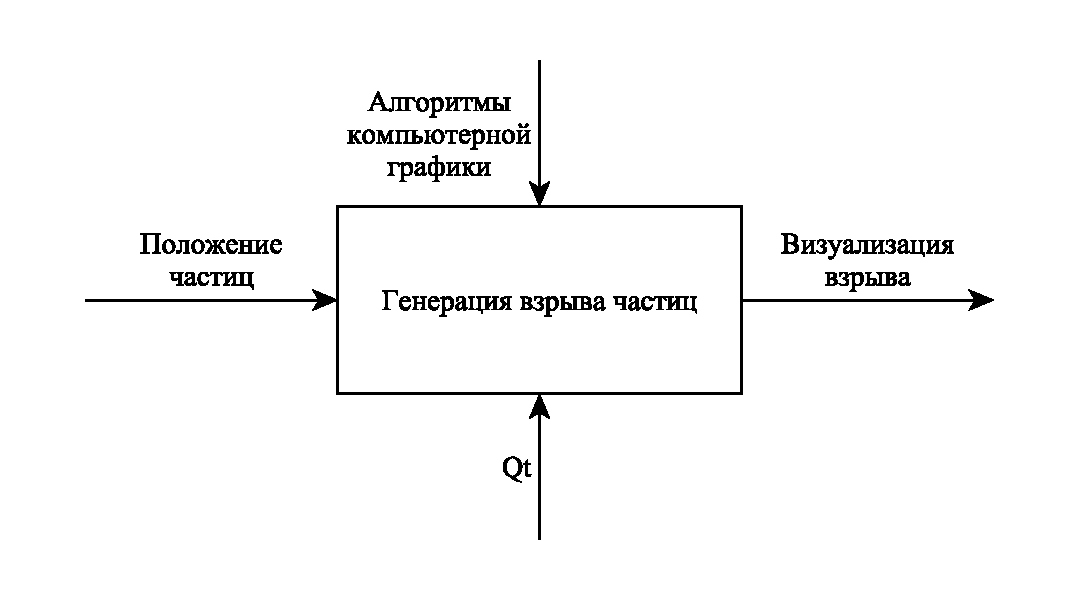
\includegraphics[scale=0.9]{idef0}
	\caption{Функциональная модель процесса визуализации взрыва частиц}
	\label{img:idef0}
\end{figure}

На вход принимаются частицы с различными параметрами (положение, масса, размер) и положение шарообразного врезающегося тела, с идентичными параметрами. На выходе получаем визуализацию взрыва мелких частиц при столкновении с телом. 

В рамках данного исследования существует возможность, менять параметры частиц. 

Ставится задача получения визуализации взрыва в режиме реального времени. 

\section{\textbf{Обзор и анализ существующих решений, обоснование необходимости разработки}}

\textbf{В настоящее время при 3D моделировании объекты часто создают в основном только двумя способами.} \cite{3dgraphic}
\begin{enumerate}
	\item Либо с помощью плоских полигонов — тем самым будет создана полая модель без внутреннего наполнения. 
	\item Либо с помощью частиц, которые полностью заполняют внутренности модели, где каждая частица представляется как материальная точка с дополнительными атрибутами, такими как скорость, цвет, ориентация в пространстве, угловая скорость и т. п.
\end{enumerate}

Ввиду того, что полигональные модели пусты по своей природе, очень трудно моделировать их поведение в 3D мире, как, например, всплески воды. Если же воду моделировать через систему чпстиц, то всё становится гораздо проще, так как вся вода от поверхности океана и до дна состоит из атомов, которые можно рассматривать, как набор отдельных частиц.

\textbf{Далее рассматриваются алгоритмы удаления невидимых поверхностей. } \cite{deletenovisible}

\begin{enumerate}
	\item Алгоритм, использующий z-буфер
	\item Алгоритм разбиения области Варнока
	\item Метод трассировки лучей
\end{enumerate}

\textbf{Алгоритм удаления поверхностей с Z-буфером. }

Алгоритм предложен Эдом Кэтмулом и представляет собой обобщение буфера кадра. Обычный буфер кадра хранит коды цвета для каждого пиксела в пространстве изображения. Идея алгоритма состоит в том, чтобы для каждого пиксела дополнительно хранить еще и координату Z или глубину. При занесении очередного пиксела в буфер кадра значение его Z-координаты сравнивается с Z-координатой пиксела, который уже находится в буфере. Если Z-координата нового пиксела больше, чем координата старого, т.е. он ближе к наблюдателю, то атрибуты нового пиксела и его Z-координата заносятся в буфер, если нет, то ни чего не делается. Таким образом, после выполнения этих операций в каждой точке экрана будет находиться пиксель, соответствующий грани, находящейся ближе всего к картинной плоскости в данной точке.

Этот алгоритм наиболее простой из всех алгоритмов удаления невидимых поверхностей, но требует большого объема памяти. Время работы алгоритма не зависит от сложности сцены. Многоугольники, составляющие сцену, могут обрабатываться в произвольном порядке. 

Основной недостаток алгоритма с Z-буфером - дополнительные затраты памяти. Другие недостатки алгоритма с Z-буфером заключаются в том, что так как пикселы в буфер заносятся в произвольном порядке, то возникают трудности с реализацией эффектов прозрачности или просвечивания и устранения лестничного эффекта. 

\textbf{Алгоритм разбиения области Варнока. }

Алгоритм работает в пространстве изображения и анализирует область на экране дисплея (окно) на наличие в них видимых элементов. Если в окне нет изображения, то оно просто закрашивается фоном. Если же в окне имеется элемент, то проверяется достаточно ли он прост для визуализации. Если объект сложный, то окно разбивается на более мелкие, для каждого из которых выполняется тест на отсутствие и/или простоту изображения. Рекурсивный процесс разбиения может продолжаться до тех пор пока не будет достигнут предел разрешения экрана (1 пиксель).

Можно выделить 4 случая взаимного расположения окна и многоугольника (рис. \ref{img:varnok}):
\begin{enumerate}
	\item многоугольник целиком вне окна,
	\item многоугольник целиком внутри окна,
	\item многоугольник пересекает окно,
	\item многоугольник охватывает окно.
\end{enumerate}

\begin{figure}[H]
	\centering
	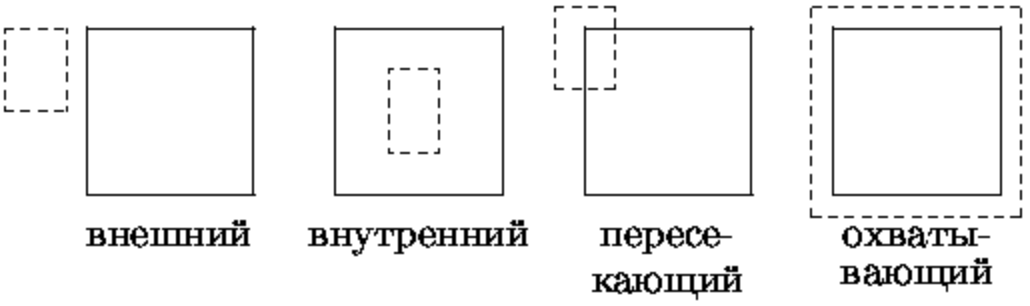
\includegraphics[scale=0.7]{varnok}
	\caption{Соотношения между окном экрана (сплошная рамка) и многоугольником (штриховая рамка)}
	\label{img:varnok}
\end{figure}

В четырех случаях можно сразу принять решение о правилах закраски области экрана:
\begin{enumerate}
	\item все многоугольники сцены - внешние по отношению к окну. В этом случае окно закрашивается фоном;
	\item имеется всего один внутренний или пересекающий многоугольник. В этом случае все окно закрашивается фоном и затем часть окна, соответствующая внутреннему или пересекающему окну закрашивается цветом многоугольника;
	\item имеется единственный охватывающий многоугольник. В этом случае окно закрашивается его цветом.
	\item имеется несколько различных многоугольников и хотя бы один из них охватывающий. Если при этом охватывающий многоугольник расположен ближе остальных к наблюдателю, то окно закрашивается его цветом.
\end{enumerate}
В любых других случаях процесс разбиения окна продолжается.

Алгоритм работает с многоугольниками. 

\textbf{Алгоритм трассировки лучей. }

Суть метода заключается в том, что для каждой точки на проектируемой плоскости строится луч, начало которого совпадает с положением наблюдателя, а угол луча по отношению к направлению наблюдения определяется характеристиками наблюдателя (максимальный угол зрения относительно горизонтальной и вертикальной плоскостей) и точкой плоскости проецирования (картинная плоскость), для которой строится луч. 

После построения луча определяется его пересечение со всеми гранями, из которых состоит сцена и выбирается та грань, расстояние от которой до наблюдателя минимально.

 Далее в данной точке картинной плоскости рисуется пиксель цветом, определяемым в точке пересечения луча и выбранной грани. 
 
 Этот метод является довольно простым и позволяет совместить определение видимости с расчётом цвета соответствующего пикселя. Ещё одним преимуществом метода является то, что сцена может состоять не из треугольников, а быть задана набором геометрических примитивов (например, поверхностями второго порядка). В этом случае пересечение луча с геометрическим примитивом вычисляется аналитически (точное решение задачи построения геометрического примитива), в отличие от разбивания произвольного геометрического примитива (например, сферы) на треугольники и решения более простой задачи пересечения луча с треугольником. 
 
 Могут генерироваться новые лучи внутри сцены для корректного отображения отражений, преломлений, затенений -- алгоритм обратной трассировки лучей более эффективен.
 
Может быть модифицирован для отображения общего освещения сцены. 

Тем не менее для реализации метода требуется довольно большое количество вычислений и следовательно большие временные затраты. 


\textbf{Актуальность темы} исследования обусловлена тем, что за последние несколько лет технология виртуальной реальности совершила огромный скачок в развитии и расширении сфер применения. Если раньше эта технология в основном применялась в военной промышленности и компьютерных играх, то сейчас виртуальная реальность проникает практически во все сферы деятельности человека: медицину, образование, архитектуру, рекламу и прочее. Эта технология имеет огромный потенциал и поэтому она так активно развивается.

\section{\textbf{Выбор, обоснование метода моделирования и алгоритма}}

На основании предложенных методов моделирования, в данной работе будет использоваться система частиц (а именно сфер). 

Для удаления невидимых поверхностей будет реализован алгоритм обратной трассировки лучей, несмотря на вычислительную сложность, алгоритм предоставляет возможность работать непосредственно со сферическими поверхностями и отображать освещение. 

\section{\textbf{Вывод}}

В данной работе ставится задача визуализации взрыва системы частиц при столкновении с шарообразным телом, используя алгоритм обратной трассировки, как наиболее оптимальный для поставленной задачи. 

На сцене располагается неподвижная, в начальный момент, группа частиц, расположенных вместе, шарообразное подвижное тело, точечный источник света.
	
В начальный момент времени, есть возможность скорректировать размеры тела, поменять расположение камеры.
	
После нажатия на кнопку, произойдёт симуляция.
\chapter{\textbf{Конструкторский раздел}}

\hfill

После запуска программы загружается модель объекта из файла в формате txt, выполняется генерация начальной картинки, устанавливаются начальные параметры (поворот камеры, размеры объектов), и после нажатия кнопки «Старт» начинается визуализация взрыва. Во время работы программы пользователь может изменять положение камеры, рассматривая модель с разных точек. 

\section{\textbf{Математические основы метода математического моделирования}}

\hfill

Для удаления невидимых поверхностей выбран алгоритм обратной трассировки лучей. А для реализации взрыва, была выбрана система частицы сферической формы. 

\subsection{\textbf{Трассировка лучей}}

\hfill

Во-первых, требуется задать точку обзора — это место, в котором располагается глаз, оно обычно называется положением камеры. Обозначим положение камеры $O(O_x, O_y, O_z)$. 

Во-вторых, в начальный момент ориентация камеры направлена вдоль положительной оси Z, положительная ось Y направлена вниз, а положительная ось X --- вправо, представлено на рисунке \ref{img:coords}. 

\begin{figure}[H]
	\centering
	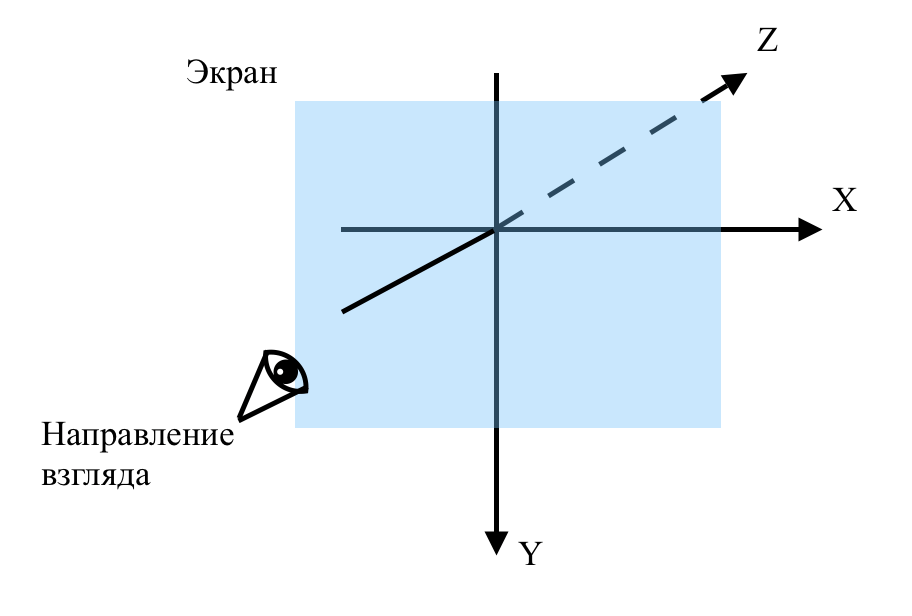
\includegraphics[scale=0.8]{coords}
	\caption{Экранная система координат с позицией камеры в начальный момент. }
	\label{img:coords}
\end{figure}

Экран - прямоугольник, называется окном просмотра. В сущности, на холсте отображается всё то, что видим через окно просмотра.

Далее необходимо определить для каждого пикселя окна просмотра ($V$) какого же он цвета.

В реальном мире свет исходит из источника света (солнца, лампочки и т.д.), отражается от нескольких объектов и наконец достигает наших глаз. Необходимо трассировать лучи «в обратном порядке» --- следует начать с луча, находящегося на камере, проходящего через точку в окне просмотра и двигаясь, пока он не столкнётся с каким-нибудь объектом в сцене. Этот объект будет «виден» из камеры через эту точку окна просмотра. То есть в качестве первого приближения следует взять цвет этого объекта как «цвет света, прошедшего через эту точку».
Алгоритм представлен на рисунке \ref{img:raytrace}. 

\begin{figure}[H]
	\centering
	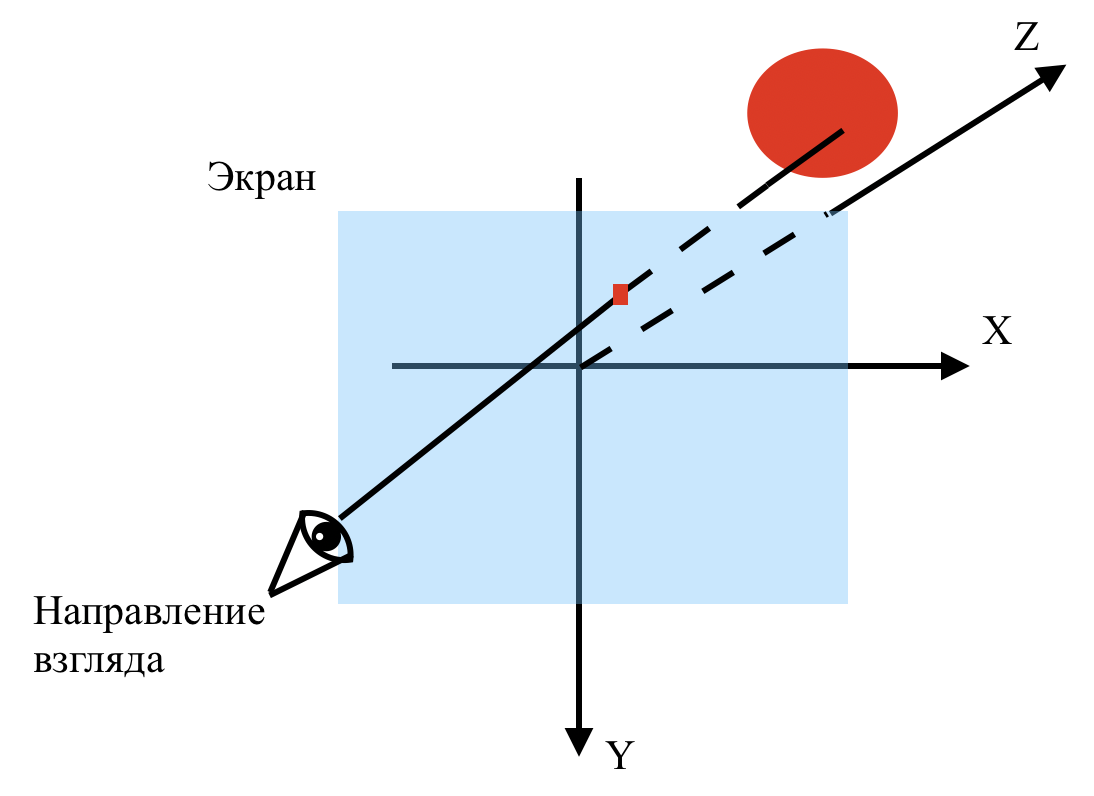
\includegraphics[scale=0.7]{raytrace}
	\caption{1 шаг алгоритма трассировки лучей. }
	\label{img:raytrace}
\end{figure}

Наилучшим способом представления лучей для поставленной цели будет использование параметрического уравнения. Луч проходит через $O$, и его направление (из $O$ в $V$), поэтому любую точку $P$ луча можно представить как $P = O + t \cdot (V - O)$, где $t$ --- произвольное действительное число. 

Обозначим направление луча за $\vec d = \overrightarrow{(V - O) }$. Тогда уравнение примет вид: $\vec p = \vec o + t\vec d$. 

Следующим шагом необходимо рассмотреть объекты сцены, с которыми лучи сталкиваются. В сцене присутствуют сферы и плоскость.

Для нахождения точки пересечения луча с произвольной поверхностью необходимо знать аналитические уравнения, определяющие оба эти объекта в трехмерном пространстве. Точка пересечения удовлетворяет всем уравнениям, так как принадлежит и лучу, и поверхности. Поэтому, сводя уравнения в систему и находя ее решения, мы получаем координаты этой точки. 

\textbf{Пересечение со сферой}

Пусть из точки $O$ выпущен луч в направлении $\vec d$, как показано на рисунке \ref{img:sphera}. 

\begin{figure}[H]
	\centering
	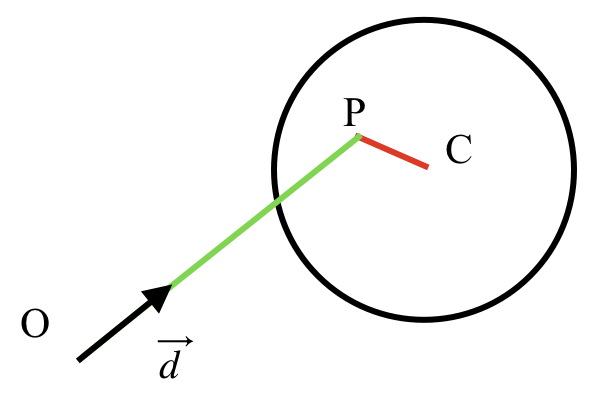
\includegraphics[scale=0.7]{sphera}
	\caption{Пересечение луча со сферой. }
	\label{img:sphera}
\end{figure}

Точкой пересечения луча и сферы является $P$ --- решение системы  \ref{eq:sphera}. 

\begin{equation}
	\centering
	\begin{cases}
   		\vec p = \vec o + t\vec d\\
   		(\vec p- \vec c)^2 = r^2
 	\end{cases}
	\label{eq:sphera}
\end{equation}

$$(\vec o + t\vec d - \vec c) ^ 2 = r^2$$
$$\text{Обозначим }\vec s = \vec c - \vec a  \text{, тогда }$$
$$(t\vec d -\vec s)^2 = r^2$$
$$t^2 \vec d^2  - 2  t \cdot (\vec d, \vec s) + \vec s ^2 = r^2$$, где $(d,s)$ — скалярное произведение $\vec d $ и$ \vec s$, равное сумме попарных произведений их координат.

Получилось квадратное уравнение \ref{eq:sqr}. 

\begin{equation}
	\centering
	D = (\vec d, \vec s)^2- \vec d^2 (\vec s ^2- r^2)
	\label{eq:sqr}
\end{equation}

Если $D < 0$, то луч проходит мимо сферы, если же $D \ge 0$, то уравнение имеет действительные корни \ref{eq:roots}. 

\begin{equation}
	\centering
	t_{1,2}=\frac{(\vec d, \vec s) \pm \sqrt{D} }{\vec d^2}
	\centering
	\label{eq:roots}
\end{equation}

Наименьшее положительное значение $t$, если оно существует, дает ответ задачи. Если же положительного значения нет, то луч сферу не пересекает.

Если точка пересечения найдена, то нас будет интересовать также нормаль к поверхности в этой точке, так как эта нормаль определяет направление отраженного луча, формула \ref{eq:normalsphere}. 

\begin{equation}
	\centering
   		\vec n = \frac{\vec p - \vec o}{|\vec p - \vec o|}
	\label{eq:normalsphere}
\end{equation}

\textbf{Пересечение с плоскостью}

Плоскость задается общим уравнением: $(\vec p, \vec n) = r$, где $\vec n$ --- вектор нормали с плоскости, имеющий единичную длину, а $r$ --- расстояние от начала координат до плоскости (с точностью до знака). См. рисунок \ref{img:plane}. 

\begin{figure}[H]
	\centering
	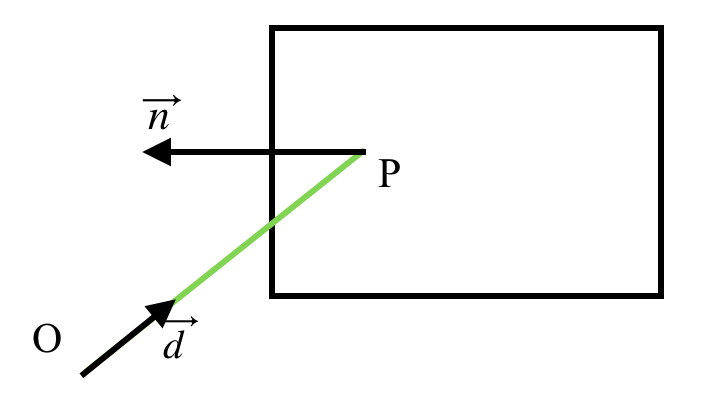
\includegraphics[scale=0.7]{plane}
	\caption{Пересечение луча с плоскостью. }
	\label{img:plane}
\end{figure}

Точкой пересечения луча и плоскости является $P$ --- решение системы  \ref{eq:plane}. 

\begin{equation}
	\centering
	\begin{cases}
   		\vec p = \vec o + t\vec d\\
   		(\vec p, \vec n) = r
 	\end{cases}
	\label{eq:plane}
\end{equation}

Тогда решением будет \ref{eq:otvet}. 

\begin{equation}
	\centering
	t = \frac{r - (\vec o, \vec n)}{(\vec d, \vec n)}
	\label{eq:otvet}
\end{equation}

Если $((\vec d, \vec n)= 0$, то луч параллелен плоскости, т.е. не пересекает ее. Если же $(\vec d, \vec n) \ne 0$, то вычисляем t. Тогда если его значение положительно, то луч пересекает плоскость.

\textbf{Источники освещения}

Свет должен откуда-то поступать. 

Точечный источник испускает свет из фиксированной точки в пространстве, называемой его позицией. Свет испускается равномерно во всех направлениях; именно поэтому его также называют всенаправленным освещением. Следовательно, точечный источник полностью характеризуется его позицией и яркостью.

Тогда $\vec l$ --- направление из точки $P$ в сцене к источнику освещения $Q$. Этот вектор, называемый световым вектором, просто равен  $\overrightarrow{Q-P}$. 

Для вычисления освещённости точки нам просто нужно вычислить количество света, вносимое каждым источником и сложить их, чтобы получить одно число, представляющее общее количество полученного точкой освещения. Затем необходимо вычислить новое значение цвета пикселя, используя цветовую модель HSV (англ. Hue, Saturation, Value — тон, насыщенность, значение). 

\textbf{Диффузное рассеяние}

Когда луч света падает на матовый объект, то из-за неровностей его поверхности, он отражает луч в сцену равномерно во всех направлениях, то есть получается «рассеянное» («диффузное») отражение.

С другой стороны, количество отражённого света зависит от угла между лучом света и поверхностью. Интуитивно это понятно --- энергия, переносимая лучом, в зависимости от угла должна распределиться по меньшей или большей поверхности, то есть энергия на единицу площади, отражённая в сцену, будет соответственно выше или ниже. 

Чтобы выразить это математически, используется вектор нормали. Вектор нормали, или просто «нормаль» — это вектор, перпендикулярный поверхности в какой-то точке. Также он является единичным вектором, то есть его длина равна 1. См. формулу \ref{eq:normalsphere} или уравнение плоскости. 

Итак, луч света с направлением $\vec l$ и яркостью $I$ падает на поверхность с нормалью $\vec n$. Какая часть $I$ отражается обратно на сцену. Схема диффузного отражения изображена на рисунке \ref{img:diffusion}. 

\begin{figure}[H]
	\centering
	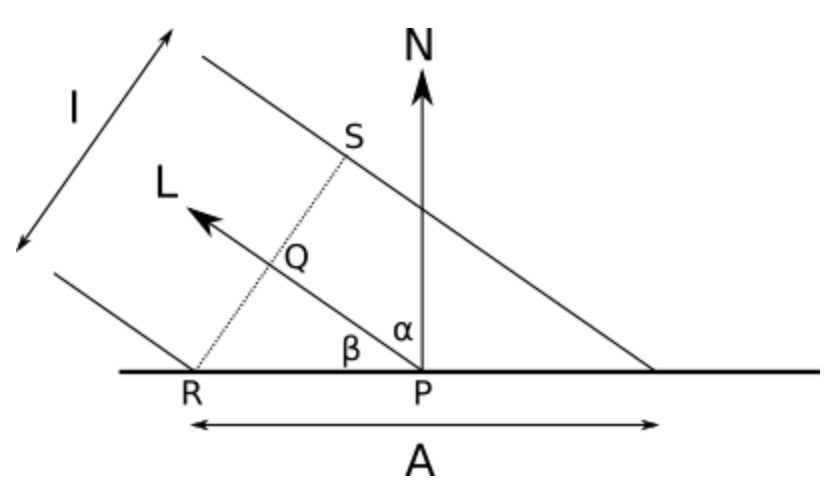
\includegraphics[scale=0.7]{diffusion}
	\caption{Диффузное отражение. }
	\label{img:diffusion}
\end{figure}

Поскольку технически луч света не имеет ширины, поэтому считается, что всё происходит на бесконечно малом плоском участке поверхности. Даже если это поверхность сферы, то рассматриваемая область настолько бесконечно мала, что она почти плоская относительно размера сферы, так же как Земля выглядит плоской при малых масштабах.

Луч света с яркостью $I$ падает на поверхность в точке $P$ под углом  $\beta$. Нормаль в точке $P$ равна $\vec n$, а энергия, переносимая лучом, распределяется по A. Нам нужно вычислить $\frac{I}{A}$.

Будем считать $SR$ «шириной» луча. По определению, она перпендикулярна $\vec l$, который также является направлением $PQ$. Поэтому $PQ$ и $QR$ образуют прямой угол. 

Давайте рассмотрим треугольник $PQR$, стороны которого связаны соотношением \ref{eq:sides}. 

\begin{equation}
	\centering
	QR = \frac{I}{2}
	\label{eq:sides}
\end{equation}

	$$PR = \frac{A}{2}$$

Тогда угол между $\vec n$ и $\vec l$ определяется по формулам \ref{eq:angle}. 

\begin{equation}
	\centering
	\cos{\alpha} = \frac{QR}{PR} = \frac{I}{A}
 	\label{eq:angle}
\end{equation}

$$\cos{\alpha} = \frac{(\vec n, \vec l)}{|\vec n||\vec L|}$$

\textbf{Тени}

Тени появляются там, где есть свет, но его лучи не могут достичь объекта, потому что на их пути есть другой объект.

Рассматривается луч, который проходит из точки до источника освещения. Пересекает ли этот луч другой объект? Если нет, то между точкой и источником ничего нет, то есть мы можем вычислить освещённость от этого источника и прибавить его к общей освещённости. Если пересекает, то мы игнорируем этот источник. См. рисунок \ref{img:shadows}. 

\begin{figure}[H]
	\centering
	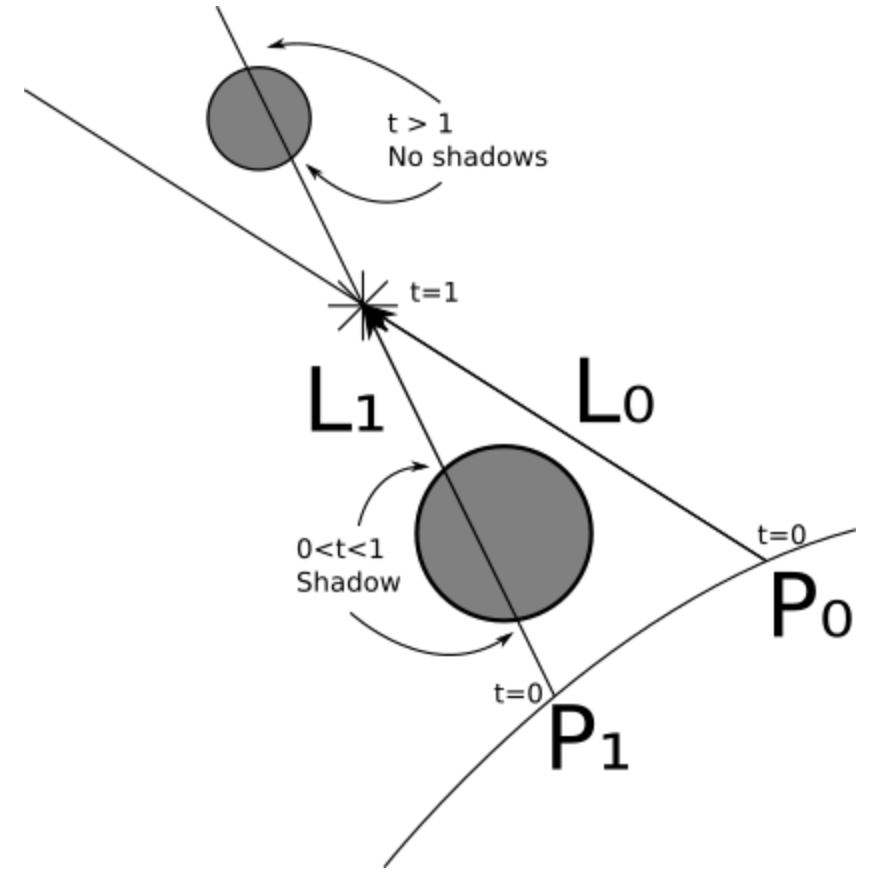
\includegraphics[scale=0.7]{shadows}
	\caption{Тени. }
	\label{img:shadows}
\end{figure}

Существует один пограничный случай, который нам нужно рассмотреть. Если искать пересечения, начиная с $t=0$, то мы, вероятнее всего, найдём саму $P$, другими словами, каждый объект будет отбрасывать тени на самого себя. 

Простейший способ справиться с этим — использовать в качестве нижней границы значений $t$ вместо 0 использовать малое значение $\epsilon$. 

\subsection{\textbf{Моделирование взрыва}}

\hfill

Взрыв частиц состоит из взаимодействия между каждой парой частиц. Приведенное ниже столкновение является описанием события 3D-столкновения и обеспечивает сохранение импульса и энергии.

Рассматриваются 2 частицы $m1,~ m2$ с радиусами $r1,~r2$, центры которых находятся в точках с координатами $(x1,~y1,~z1),~(x2,~y2,~z2)$ и двигаются со скоростями $(vx1,~vy1,~vz1),~(vx2,~vy2,~vz2)$. 

\textbf{Алгоритм. }
\begin{enumerate}
	\item Вычислить относительное расстояние и относительную скорость. 
	
	\item Если расстояние между шарами больше суммы радиусов или если относительная скорость = 0 (частицы не взаимодействуют) $\to$ выход из подпрограммы. 
	
	\item Для моделирования необходимо перейти в систему координат, одна из осей которой направлена вдоль вектора скорости 2 шара (он покоится), а начало координат совпадает с центром первой частицы. См. рисунок  \ref{img:coords_explosion}. 
	
	Для этого необходимо сдвинуть систему координат так, чтобы шар 1 находился в начале координат, а затем изменить скорость 1 шара на относительную (так как 2 шар покоится в новой системе отсчета). Для того чтобы ось $Z$ была направлена вдоль вектора $v_2$, необходимо сделать два поворота: первый --- на угол $\varphi$ вокруг оси Z, второй --- на угол $\theta$ вокруг оси Y.
	
	\begin{figure}[H]
		\centering
		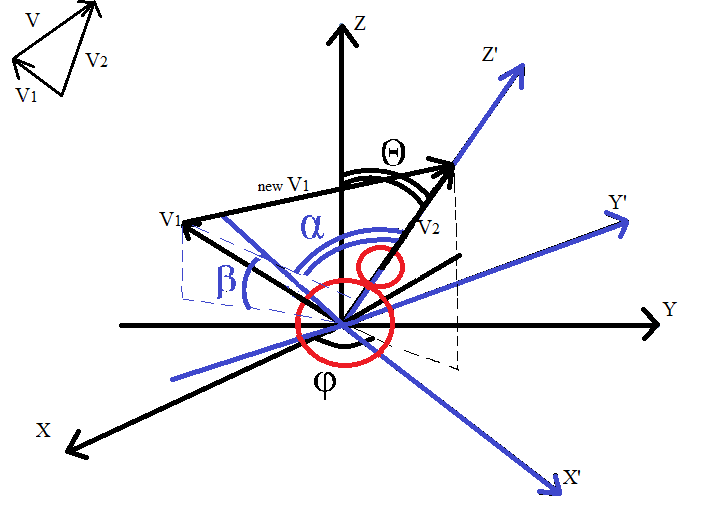
\includegraphics[scale=0.6]{coords_explosion}
		\caption{Преобразование координат. }
		\label{img:coords_explosion}
	\end{figure}
	
	Матрица первого поворота \ref{eq:matr_varphi}. 
	
	\begin{equation}
		\begin{pmatrix}
			\cos{\varphi}& \sin{\varphi} & 0\\
			-\sin{\varphi}& \cos{\varphi} & 0\\
			0&0&1
		\end{pmatrix}
		\label{eq:matr_varphi}
	\end{equation}
	
	Матрица второго поворота \ref{eq:matr_theta}. 
	
	\begin{equation}
		\begin{pmatrix}
			\cos{\theta}& 0 & -\sin{\theta}\\
			0& 1 & 0\\
			\sin{\theta}&0&\cos{\theta}
		\end{pmatrix}
		\label{eq:matr_theta}
	\end{equation}
	
	Пересчет координат вектора при переходе от системы $XYZ$ к системе $X'Y'Z'$ дается произведением матриц \ref{eq:matr_varphi}, \ref{eq:matr_theta}. 
	
	\begin{equation}
		\begin{pmatrix}
			\cos{\theta}\cos{\varphi}& \cos{\theta}\sin{\varphi} & -\sin{\theta}\\
			-\sin{\varphi}& \cos{\varphi} & 0\\
			\sin{\theta}\cos{\varphi}&\sin{\theta}\sin{\varphi}&\cos{\theta}
		\end{pmatrix}
		\label{eq:matr_rotate}
	\end{equation}
	
	Обратный переход от системы $X',Y',Z'$ к системе $XYZ$ производится с помощью транспонированной матрицы \ref{eq:matr_transpose}. 
	
	\begin{equation}
		\begin{pmatrix}
			\cos{\theta}\cos{\varphi}& -\sin{\varphi} & \sin{\theta}\cos{\varphi}\\
			\cos{\theta}\sin{\varphi}& \cos{\varphi} & \sin{\theta}\sin{\varphi}\\
			-\sin{\theta}&0&\cos{\theta}
		\end{pmatrix}
		\label{eq:matr_transpose}
	\end{equation}
	
	\item Проверить сталкиваются ли шары (пересечение векторов скоростей) $\to$ если нет, выход из-под программы. 
	\item Нахождение новых скоростей, решением системы уравнений \ref{eq:system}.  
	
	\begin{equation}
		\begin{cases}
			m_1 v_{1,x} = m_1 v_{1,x}' + m_2 v_{2,z}' \tg{\alpha}\cos{\beta}\\
			m_1 v_{1,y} = m_1 v_{1,y}' + m_2 v_{2,z}'\tg{\alpha}\sin{\beta}\\
			m_1 v_{1,z} = m_1 v_{1,z}' + m_2 v_{2,z}'\\
			\frac{m_1(v_{x,1}^2+v_{y,1}^2+v_{z,1}^2) }{2} =  \frac{m_1(v_{x,1}'^2+v_{y,1}'^2+v_{z,1}'^2)}{2} + \frac{m_2v_{z,2}'^2(1+\tg{\alpha}^2)}{2} 
		\end{cases}
		\label{eq:system}
	\end{equation}

	\item Обновить скорости и повернуть векторы скорости назад и добавить начальный вектор скорости шара 2, чтобы получить исходную систему координат. 
	
\end{enumerate}

\section{\textbf{Разработка и обоснование используемых типов и структур данных }}

В данной работе происходит взаимодействие с моделью, структура которой представлена на рисунке \ref{img:model}. Состоит из вектора частиц (система частиц, в которой каждая частица обладает определенными параметрами), земля --- плоскость, на которой происходит взаимодействие частиц и частица, рассматриваемая отдельно, в начальный момент имеющая скорость. 

\begin{figure}[H]
	\centering
	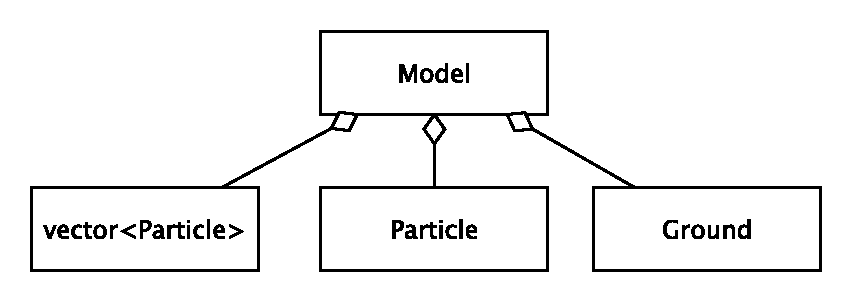
\includegraphics[scale=0.7]{model}
	\caption{Структура модели. }
	\label{img:model}
\end{figure}

Камера в данной работе содержит класс матрицы, для удобства взаимодействия. В ней реализованы методы, умножения матрицы на матрицу, вектора на матрицу для работы с преобразования координат. 

\begin{figure}[H]
	\centering
	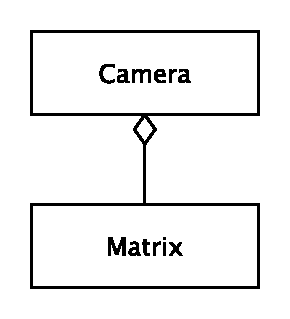
\includegraphics[scale=0.7]{camera}
	\caption{Структура камеры. }
	\label{img:camera}
\end{figure}

\section{\textbf{Разработка структуры программного комплекса}}
\hfill

Алгоритм работы программы. 
\begin{enumerate}
	\item[1. ] Загрузка модели из txt файла.
	\item[2. ] Установка первоначальных параметров для модели сцены и камеры. 
	\item[3. ] Вычисление координат и положения объекта (для различных этапов взрыва). 
	\item[4. ] Преобразование координат (повороты моделей, масштабирование и перенос) относительно камеры.
	\item[5. ] Генерация и отображение модели. 
	\item[6. ] Считывание новых параметров. 
	\item[7. ] Возвращение к п.3. 
\end{enumerate}

\section{\textbf{Вывод}}

\hfill

Необходимо реализовать алгоритмы трассировки лучей для удаления невидимых поверхностей и работы с освещением (диффузное отражение и тени). Далее необходимо разработать алгоритм визуализации взрыва с опорой на физические законы, такие как закон сохранения энергии и закон сохранения импульса. 

Необходимо также разработать взаимодействие с камерой и объектом (перемещение, масштабирование, поворот). 

\chapter{\textbf{Технологический раздел}}

\hfill

В соответствии с выбранной задачей -- визуализацией взрыва. Необходимо выбрать средства реализации, создать интерфейс и структуры программного обеспечения, описать ограничения и порядок работы программы. 

\section{\textbf{Выбор и обоснование языка программирования }}

Для выполнения проекта был выбран язык программирования C++/QT.

C++ -- компилируемый, статически типизированный язык программирования общего назначения \cite{c++}. 

C++ сочетает свойства высокоуровневого и низкоуровневого языка. В сравнении с его предшественником, языком C, присутствует поддержка объектно-ориентированного программирования.

Являясь одним из самых популярных языков программирования, C++ широко используется для разработки программного обеспечения \cite{usingc++}. 

Qt -- кроссплатформенная библиотека разработки GUI на С++ \cite{qt}.

Библиотека Qt является безусловным лидером среди имеющихся средств разработки кроссплатформенных приложений на языке C++. Qt – полностью объектно-ориентированная библиотека.

Все элементы в окне программы, кнопки, переключатели - это отдельные виджеты. Именно виджеты являются основой построения графических интерфейсов. С точки зрения программы, они воспринимают все
события и генерируют сигналы, которые в свою очередь вызывают слоты – специальные функции, реагирующие на различные события в окне. 

Qt прекрасно документирована, благодаря чему всегда можно найти о ней любую интересующую информацию.

Для написания программного кода использовался Qt Creator 4.8.1. Основная задача Qt Creator -- упростить разработку приложения с помощью фреймворка Qt на различных платформах.

\section{\textbf{Интерфейс пользователя }}

Взаимодействие пользователя с приложением осуществляется через интерфейс, представленный на рисунке \ref{img:interface}. 

\begin{figure}[H]
	\centering
	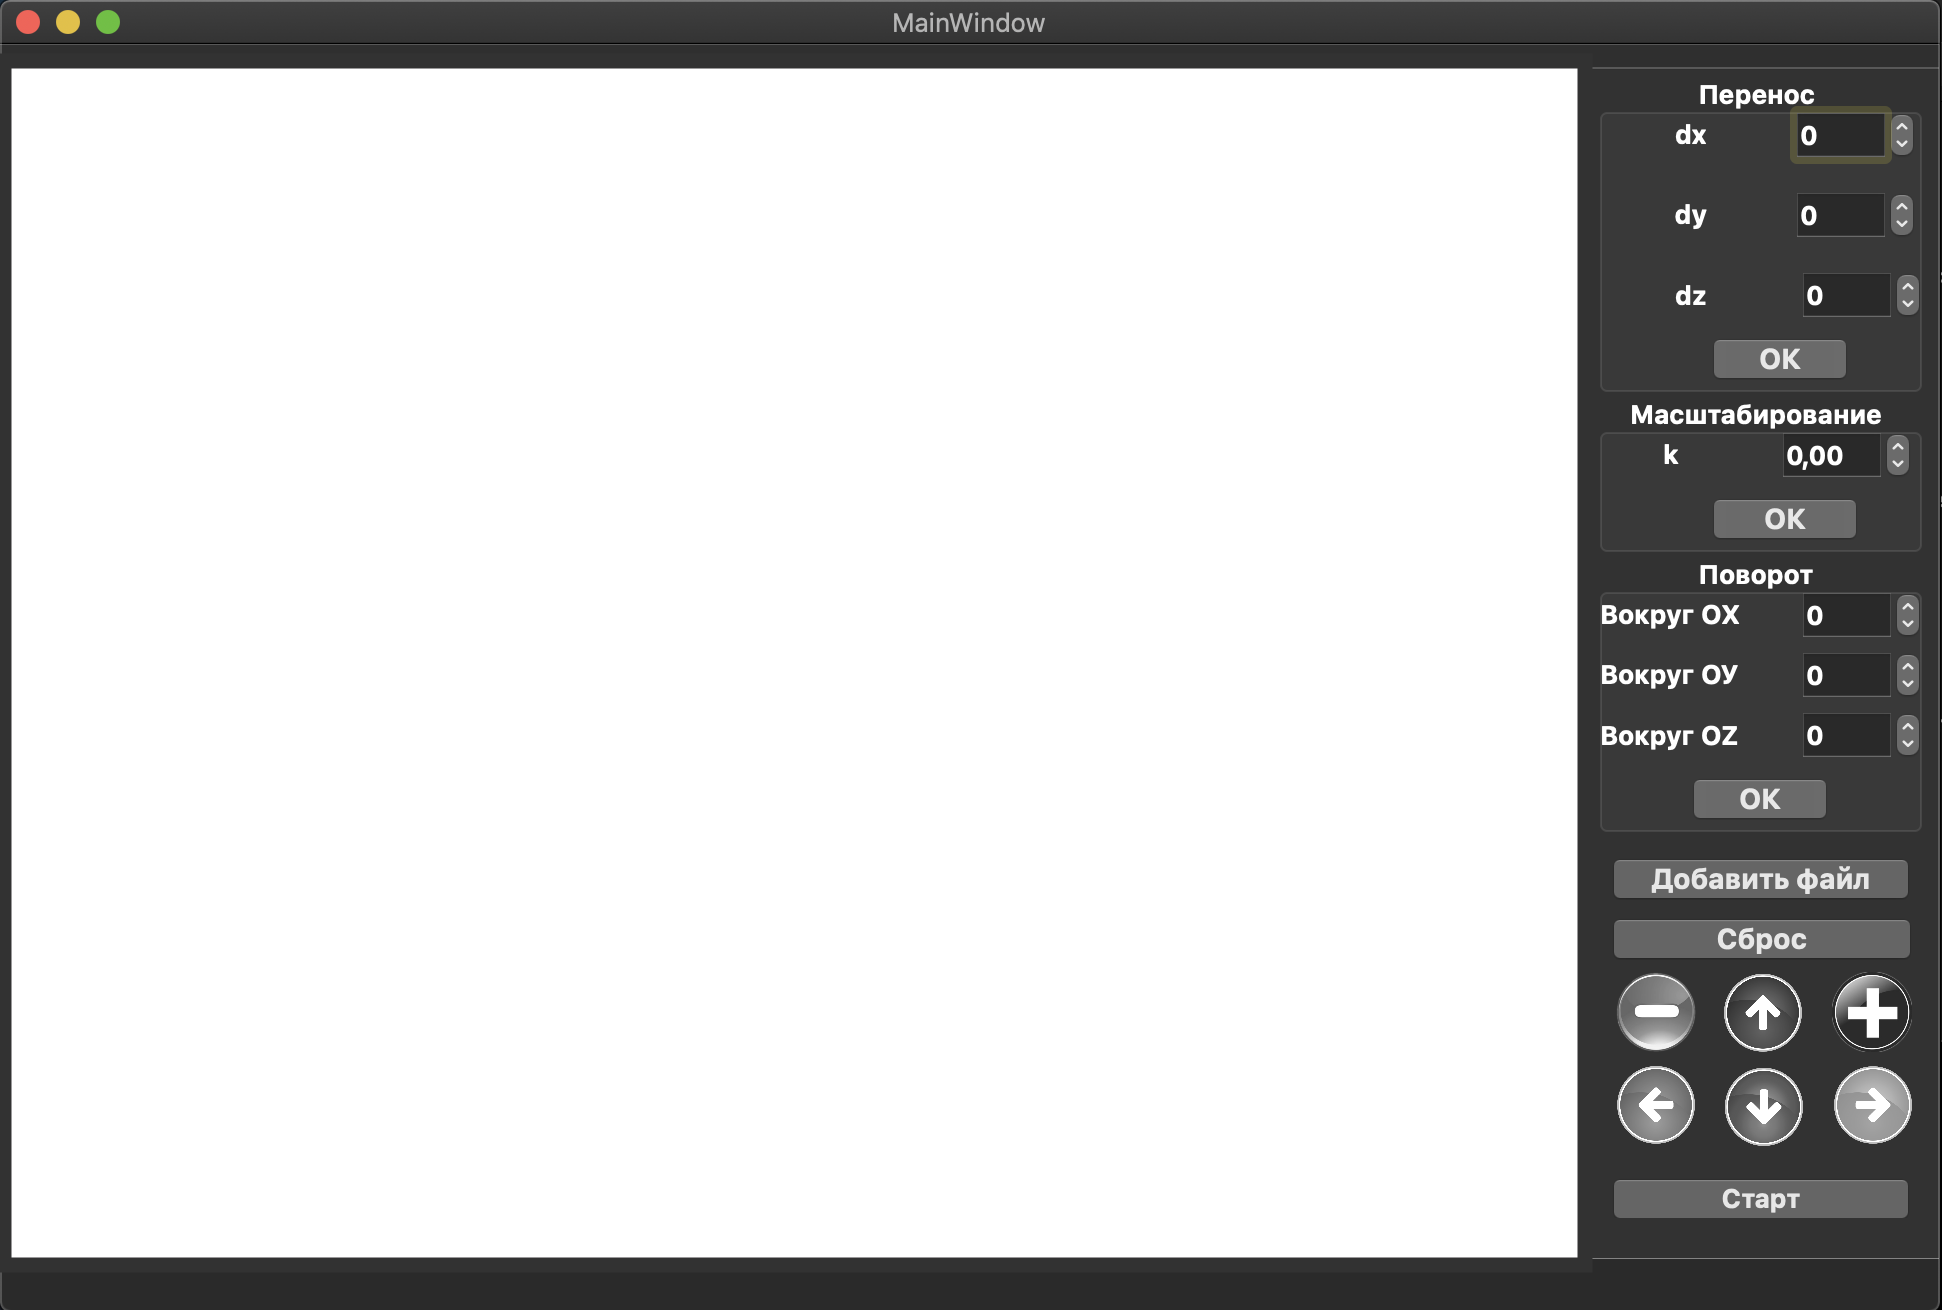
\includegraphics[scale=0.4]{interface}
	\caption{Интерфейс пользователя}
	\label{img:interface}
\end{figure}

\begin{enumerate}
	\item Доступны поля для ввода данных, при желании менять расположение и вид объектов. 
	\item Кнопки ($\to, \leftarrow, \uparrow, \downarrow, +, -$) предназначены для взаимодействия с камерой. 
	\item Кнопка  <<Сброс>> -- сбрасывает все настройки в начальное состояние. 
	\item Кнопка <<Добавить файл>> -- для загрузки данных. 
	\item Слайдер -- для задания скорости частицы в начале. 
	\item Кнопка <<Старт>> -- запускает визуализацию взрыва.   
\end{enumerate}

\section{\textbf{Хранение и обмен данными в системе }}

Данные считываются из файла, содержащего в себе:

1-я строка -- количество частиц

2 -я строка и последующие строки содержать в себе информацию о частицах: положение, радиус и вес (5 значений через пробел). 

Последняя строчка рассматривается, как частица, которая в начальный момент получит скорость движения. 

Из каждого файла считывается модель, состоящая из вектора частиц, позиции земли (плоскости ограничивающей взаимодействие). Класс частицы представлен в листинге \ref{lst:particle}. 


\begin{lstlisting}[caption=Класс частицы, label = lst:particle, style=simplecode]
class Particle
{
public:
    Particle() {}
    Particle(Point_3d point, int r, int m);
    Particle(Point_3d point, int r);
    Particle(Point_3d point);
    ~Particle() {}

    void set_p(const Point_3d p);
    Point_3d get_p() const;

    void set_v(const Point_3d v);
    Point_3d get_v() const;

    void set_m(const double m);
    double get_m() const;

    void set_r(const int r);
    int get_r() const;

    void collision(Particle &p);
    void update(int time);

private:
    Point_3d point;
    Point_3d speed;
    int m;
    int radius;
};
\end{lstlisting}

\section{\textbf{Разработка программы}}

В данной работе, используется объектно-ориентированный подход программирования и паттерны проектирования\cite{patterns}. 

Для связание интерфейса и реализации используются паттерны фасад и команда. См. рисунки \ref{img:facade}, \ref{img:commands}. 

\begin{figure}[H]
	\centering
	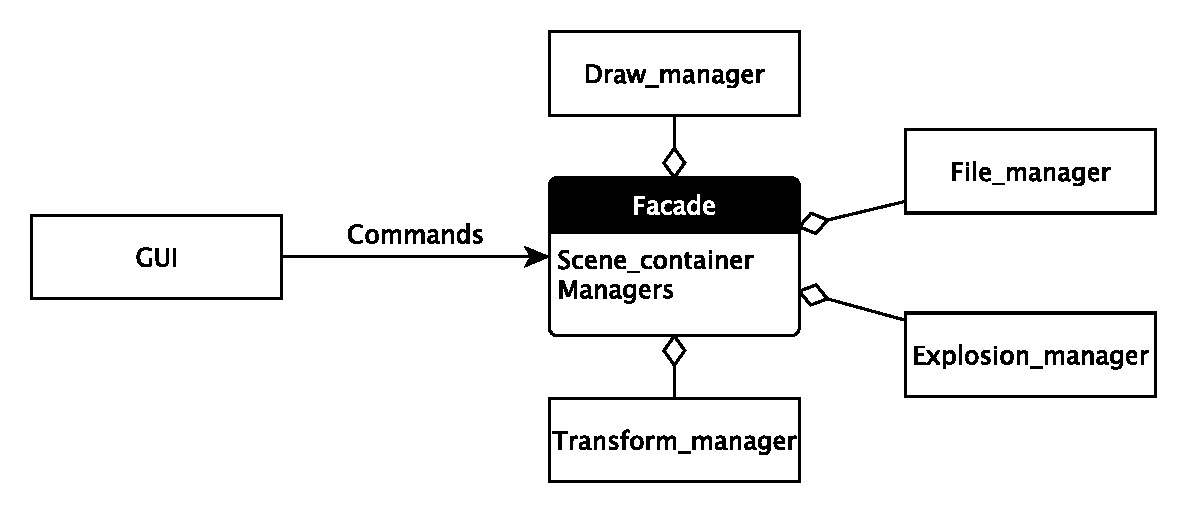
\includegraphics[scale=0.7]{facade.pdf}
	\caption{Паттерн фасад}
	\label{img:facade}
\end{figure}

\begin{figure}[H]
	\centering
	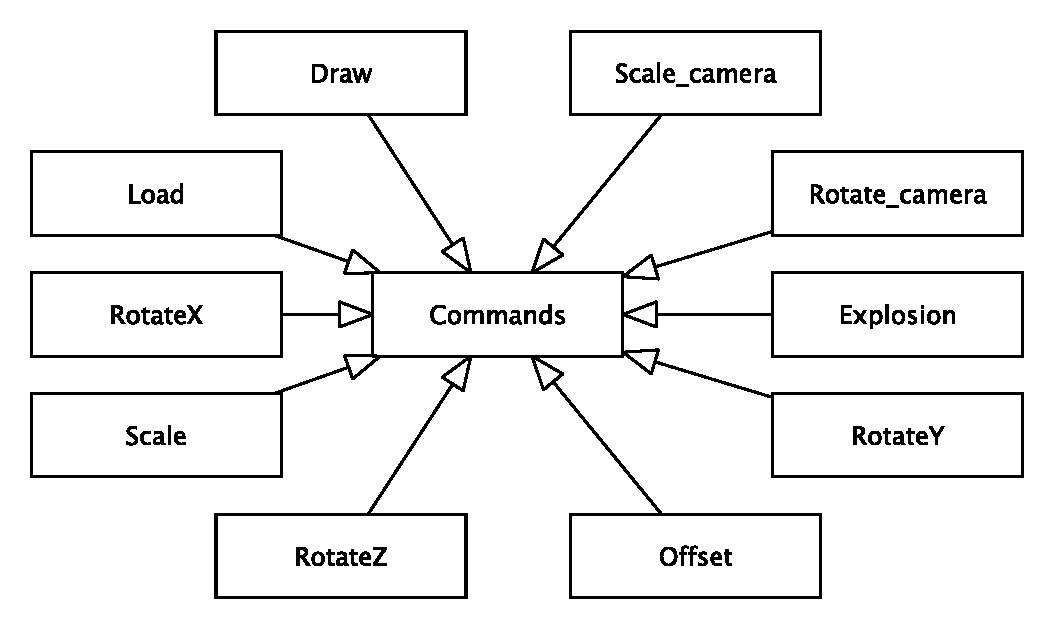
\includegraphics[scale=0.7]{commands.pdf}
	\caption{Паттер команда}
	\label{img:commands}
\end{figure}

Структура сцены в данной работе представлена на рисунке \ref{img:scenecontainer}. 

\begin{figure}[H]
	\centering
	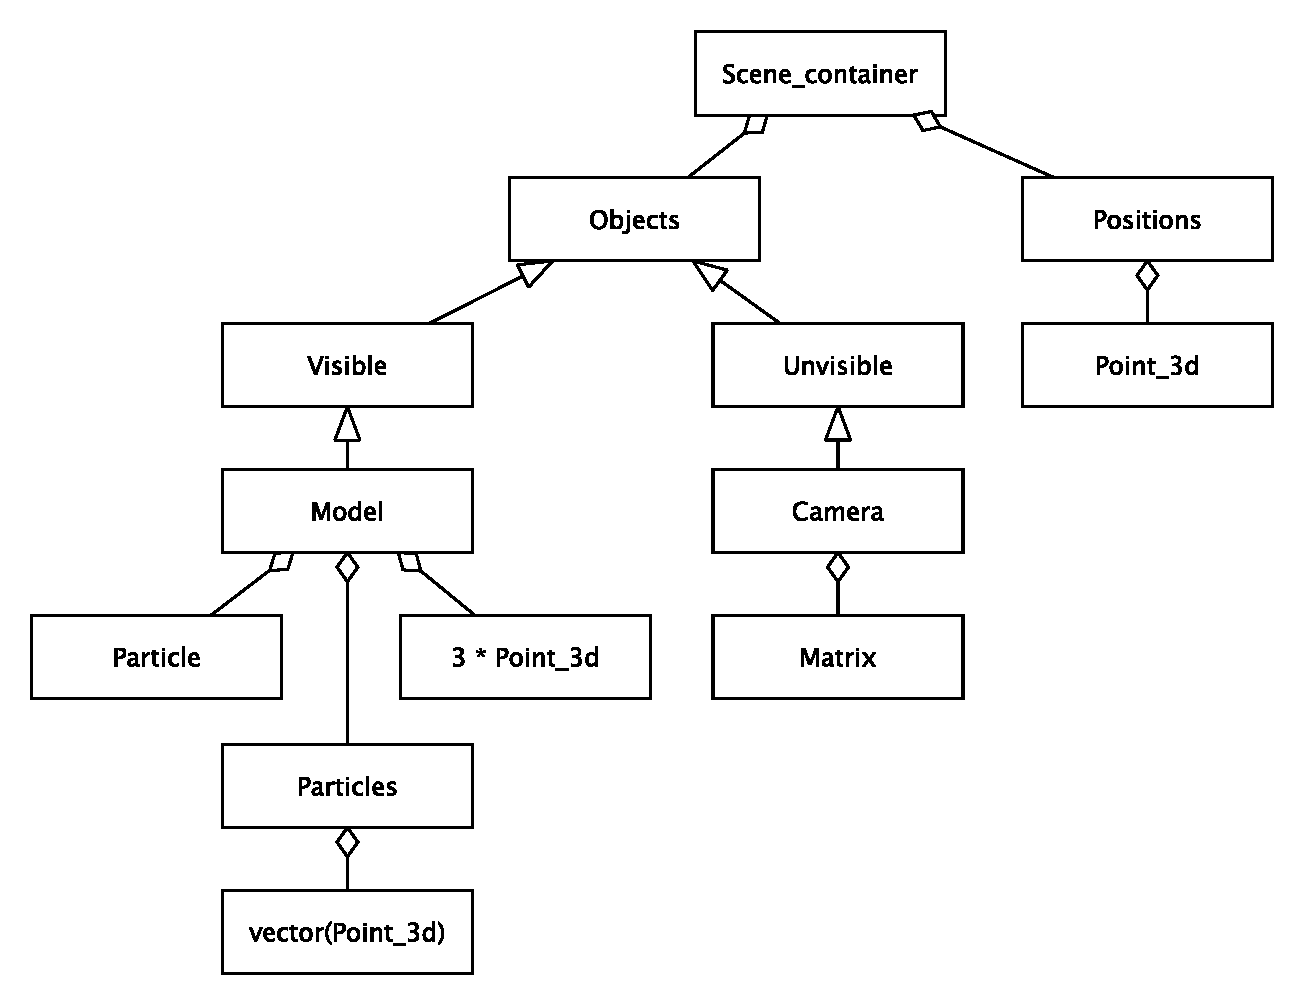
\includegraphics[scale=0.7]{scenecontainer.pdf}
	\caption{Контейнер сцены}
	\label{img:scenecontainer}
\end{figure}

Для создания сложной модели используется паттерн строитель. Для последовательного обхода объектов на сцене -- паттерн итератор. 

\section{\textbf{Требования к аппаратуре }}

Так как в данной работе используется трассировка лучей, в которой необходимо пробегаться по всем пикселям экрана, стоит необходимость уменьшения временных затрат на вычисления. 

Таким образом, существует необходимость использования параллельных вычислений. Так как параметры каждого пикселя экрана вычисляются независимо от других, то для того, чтобы вычислить все параллельно, достаточно просто указать какие пиксели какому потоку вычислять.

Теоретически, для нахождения значения каждого из пикслей можно создать свой поток. Но ОС не позволит создать такое число потоков, ресурсов на их создание не хватит и создание потока также занимает определенный промежуток времени.

Алгоритм. 
\begin{enumerate}
	\item Разделить экран по оси Х на равные участки N. 
	\item Создать N потоков с указанием вычисляемых пикселей. 
	\item Запустить потоки. 
\end{enumerate}

Проведено исследование с замером времени необходимого на отрисовку экрана для разного количества потоков. Количество повторов эксперимента -- 15.

\begin{table}[]
	\begin{tabular}{|c|l|l|l|l|l|}
	\hline
	\begin{tabular}[c]{@{}c@{}}Количество \\ потоков\end{tabular}                                  & 1           & 2       & 4          & 8          & 16         \\ \hline
	\begin{tabular}[c]{@{}c@{}}Среднее время \\ визуализации\\ экрана,\\ микросекунды\end{tabular} & 11518775.92 & 6013675 & 3298333.53 & 2843617.94 & 2886129.94 \\ \hline
	\end{tabular}
\end{table}

Как видно из эксперимента, наиболее быстрая отрисовка при количестве потоков равным 8, что равно количеству логических ядер процессора. 

Следовательно, для наиболее быстрой работе, количество логических ядер процессора на персональном компьютере должно быть больше 8. 

\section{\textbf{Требования к программному обеспечению }}

С помощью Qt можно создавать графические приложения на различных операционных системах, не переписывая исходный код. Qt поддерживается на различных 32-битных и 64-битных платформах. 

Qt -- кроссплатформенная библиотека разработки GUI на С++, а значит нет привязки к платформе, возможно использование любого ПО. 

Qt Creator доступен для следующих операционных систем:

\begin{enumerate}
	\item[1. ]Windows 7 или более поздняя версия
	\item[2. ]Ubuntu Linux 16.04 (64-разрядная версия) или более поздняя версия
	\item[3. ]macOS 10.12 или более поздней версии
\end{enumerate}

\section{\textbf{Порядок работы }}

Алгоритм программы. 

\begin{enumerate}
	\item[1. ] Визуализация начального экрана и интерфейса. 
	\item[2. ] Ввод и чтение из пользовательского файла. 
	\item[3. ] Если ошибок не возникло, загрузка новой модели. 
	\item[4. ] Визуализация модели с учетом матрицы камеры. 
	\begin{enumerate}
		\item Алгоритм трассировки для каждого пикселя экрана. 
		\item Определение затененности для каждого пикселя экрана. 
		\item Применение диффузного отражения для каждого пикселя экрана. 
		\item Отрисовка пикселей. 
	\end{enumerate}
	\item[5. ] При нажатой кнопке взрыва. 
	\begin{enumerate}
		\item Пересчет скорости каждого объекта по законам физики. 
		\item Пересчет положения каждого объекта с учетом скорости. 
	\end{enumerate}
	\item[6. ] Переход к пункту 4, если не загружен новый файл, иначе пункт 2. 
\end{enumerate}

\section{\textbf{Обращение к программе }}

Программа компилируется и запускается с помощью Qt Creator. 

Взаимодействие пользователя с приложением осуществляется через интерфейс, представленный на рисунке \ref{img:interface}. 

\section{\textbf{Входные и выходные данные }}

На вход поступают данные из файла, определенного вида. Также можно изменять данные с помощью графического интерфейса или менять направление камеры. 

На выходе получаем визуализацию столкновения частиц. 


\section{\textbf{Сообщения  системы }}

Система уведомляет пользователя в случае некорректных данных. 

\begin{enumerate}
	\item Отсутствует файл при загрузке. 
	\begin{figure}[H]
		\centering
		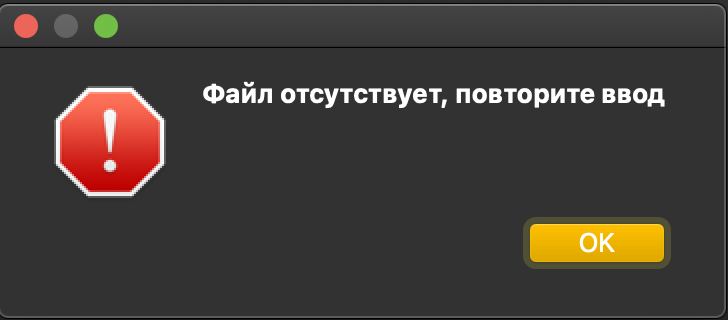
\includegraphics[scale=0.7]{nofile}
		\caption{Отсутствует файл}
		\label{img:nofile}
	\end{figure}
	\item Некорректный файл (данные в нем). 
	\begin{figure}[H]
		\centering
		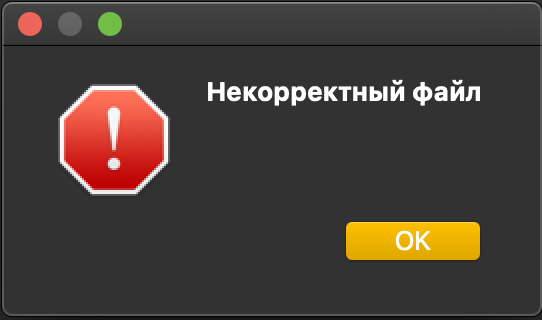
\includegraphics[scale=0.7]{incorrectfile}
		\caption{Некорректные данные в файле}
		\label{img:incorrectfile}
	\end{figure}
	\item Некорректные значения в полях ввода интерфейса. 
	\begin{figure}[H]
		\centering
		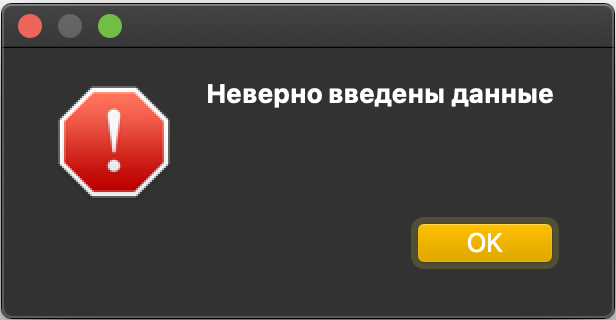
\includegraphics[scale=0.7]{incorrectdata}
		\caption{Некорректные вводимые данные}
		\label{img:incorrectdata}
	\end{figure}
\end{enumerate}

\section{\textbf{Вывод}}

В данном разделе подготовлен и отлажен исходный код приложения, приведены этапы работы приложения, способы хранения данных. Представлены и протестированы различные случаи работы приложения, как корректные так и некорректные. 

\chapter{\textbf{Экспериментальный раздел}}

Проводится анализ реализованного приложения, проверяется корректность работы, строятся графики зависимости времени генерации картинки от количества частиц и количества потоков. 

\section{\textbf{Исследование характеристик программы }}

В работе для ускорения вычислений используется параллельной программирование. Необходимо исследовать оптимальное число потоков необходимых для наиболее быстрой генерации изображения. 

Из графика, представленного на рисунке \ref{img:graph} видно, что при генерации частиц, количество которых не превышает 50, использование 4 поток наиболее эффективно, например на 15\% чем 8 потоков и в 4 раза чем при использовании 1 потока. 

Однако при росте числа частиц, ситуация меняется. Использование 8 и 16 потоков становится эффективнее, причем 8 потоков быстрее чем 16 на 3\%. 

\begin{figure}[H]
	\centering
	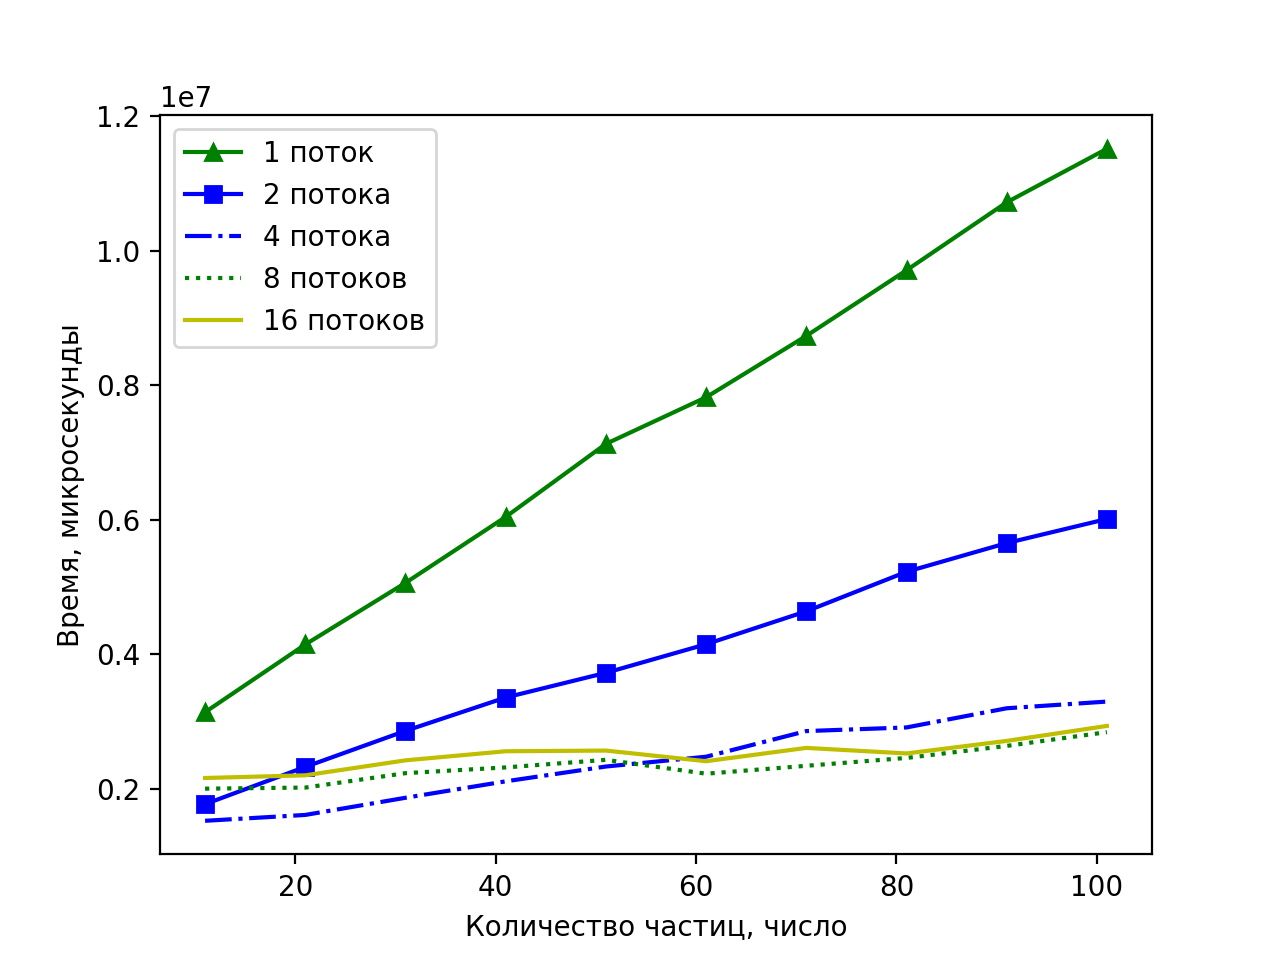
\includegraphics[scale=1]{graph}
	\caption{График зависимости времени генерации изображения от количества частиц для различного числа потоков}
	\label{img:graph}
\end{figure}

Стоит заметить, что 8 потоков соответствует количеству логических ядер процессора. 

Таким образом, получается что количество потоков будет на прямую зависеть от параметров компьютера, на котором запущена визуализация. 

\section{\textbf{Примеры использования программы }}

Примеры работы программы представлены на рисунках \ref{img:ex1}, \ref{img:ex2}. Визуализация одного и того же процесса в разные моменты времени. 

\begin{figure}[H]
	\centering
	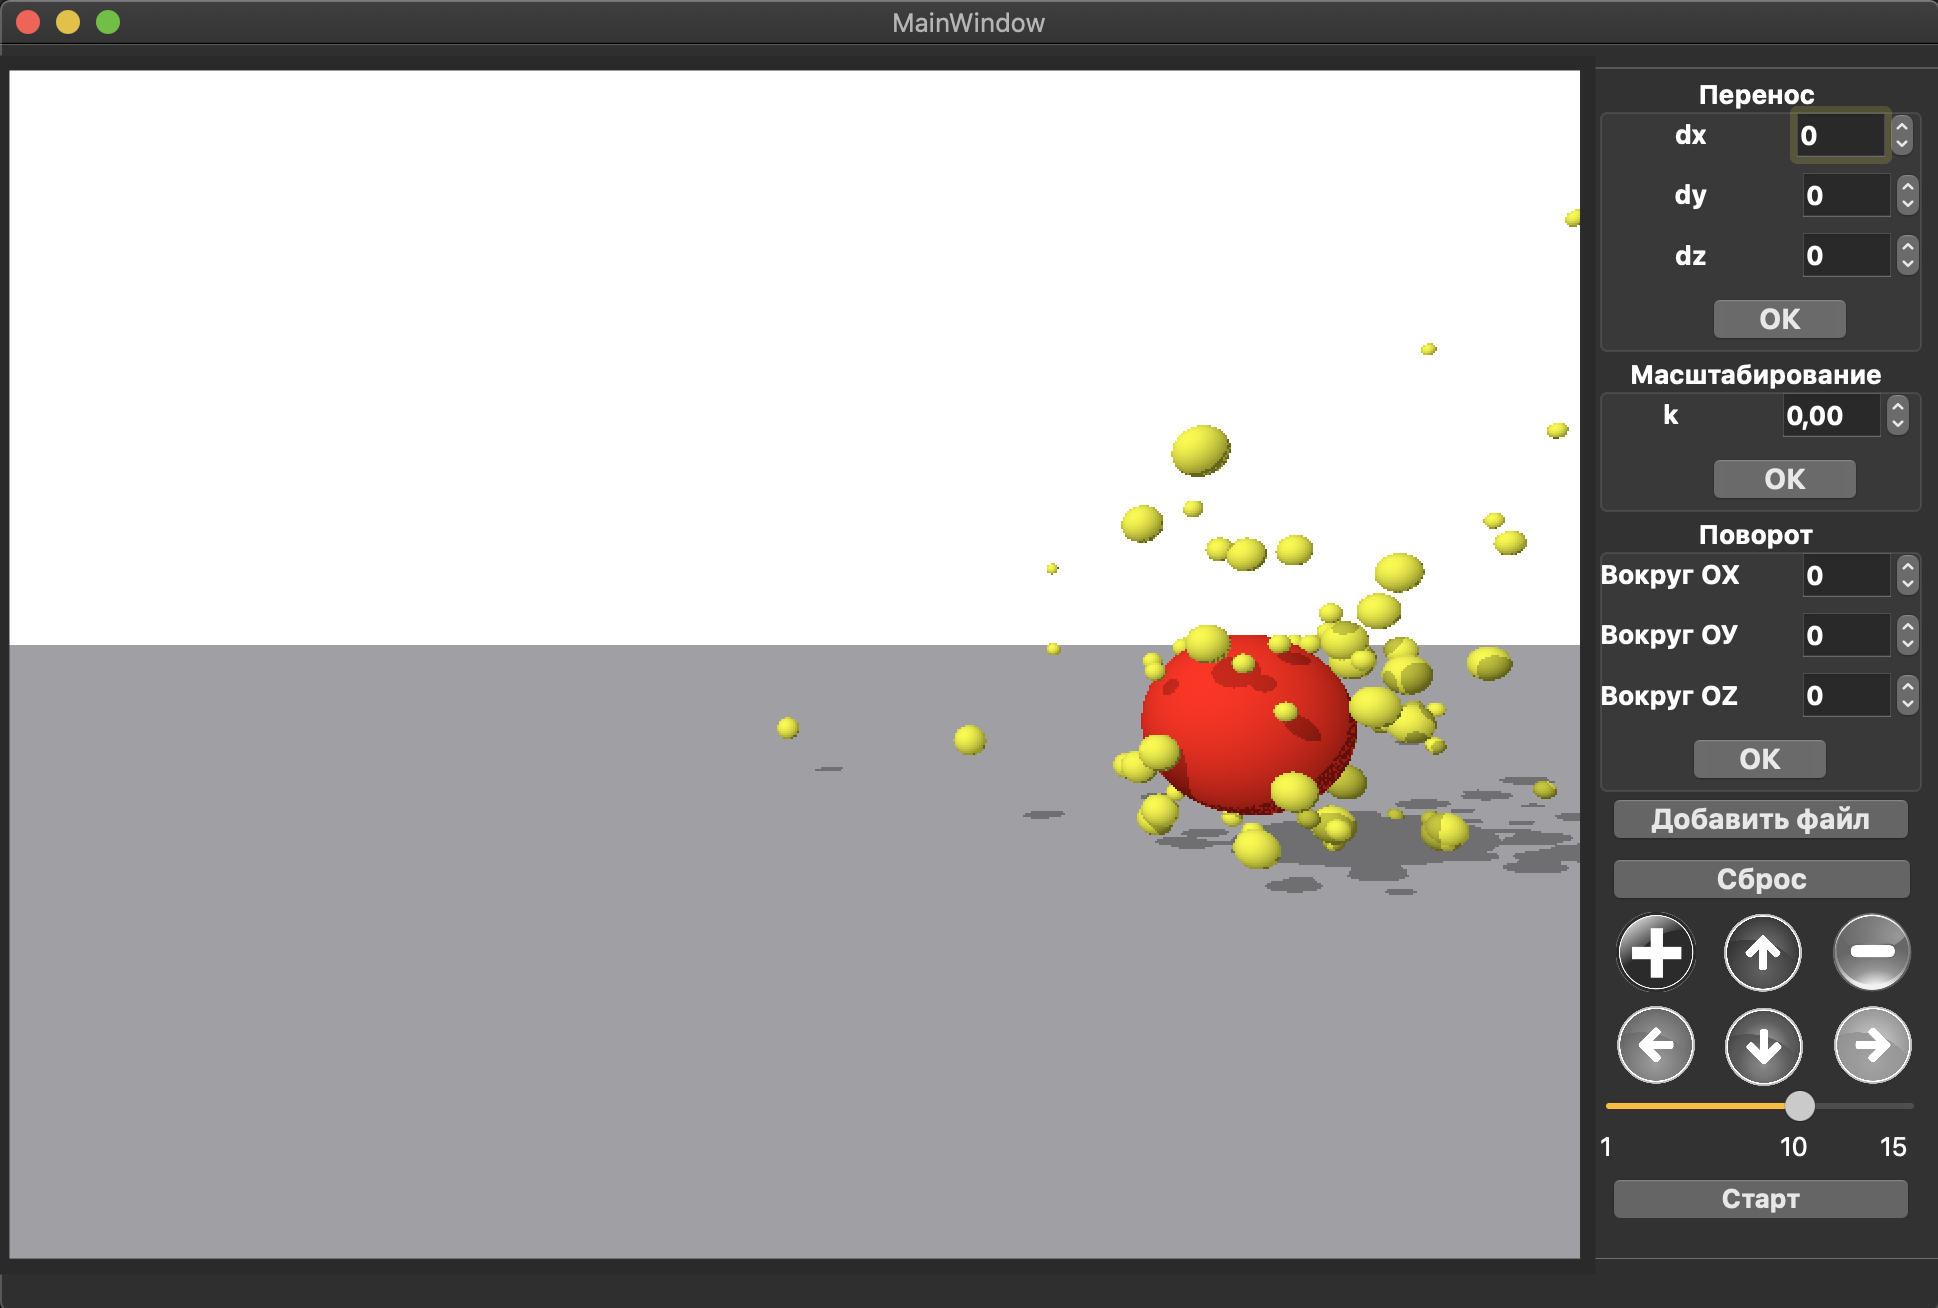
\includegraphics[scale=0.4]{ex2}
	\caption{Пример 1}
	\label{img:ex1}
\end{figure}

\begin{figure}[H]
	\centering
	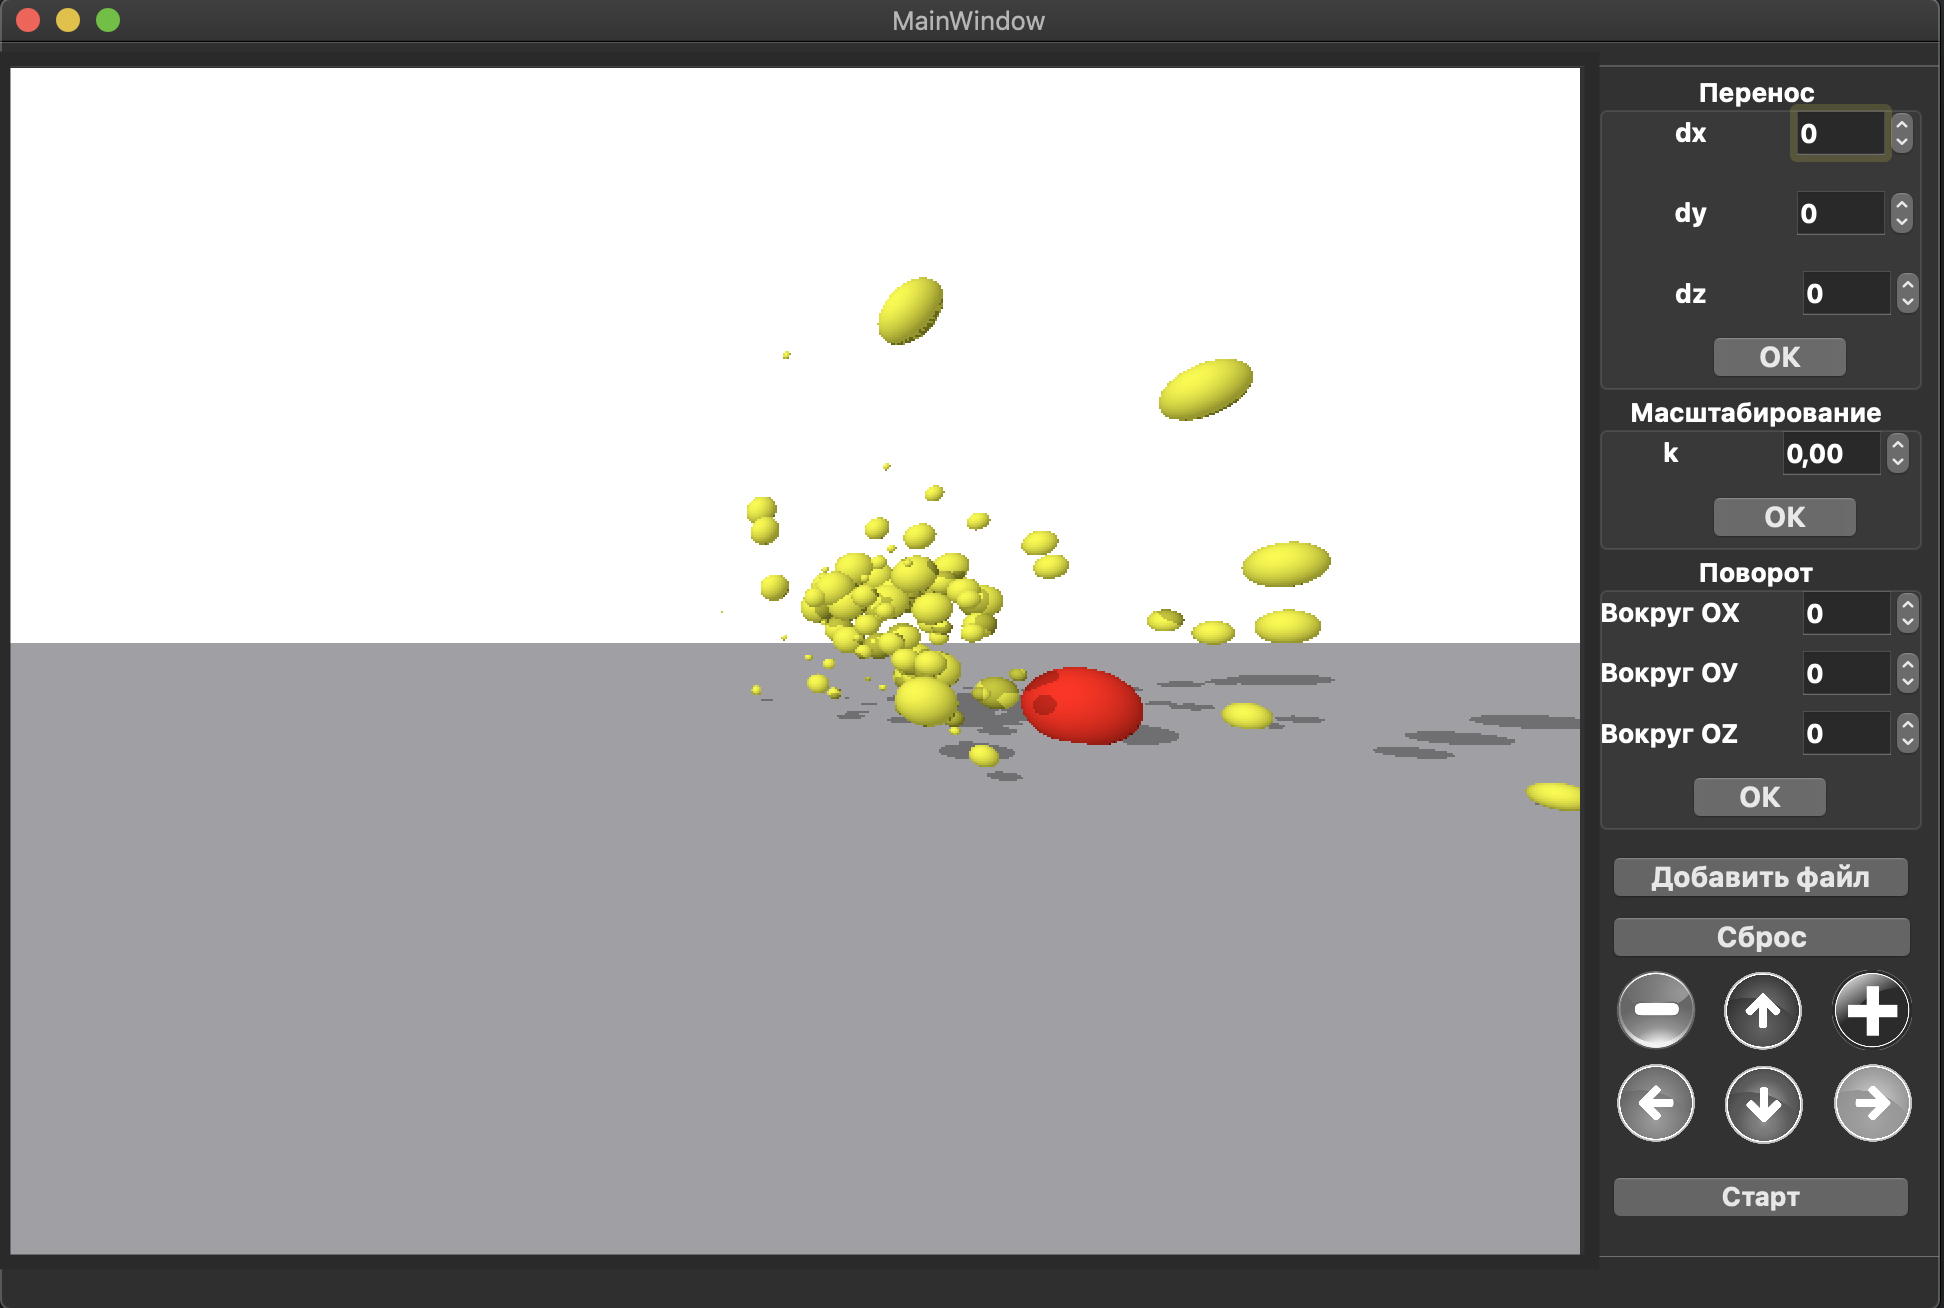
\includegraphics[scale=0.4]{ex1}
	\caption{Пример 2}
	\label{img:ex2}
\end{figure}

\section{\textbf{Вывод}}

Проведено исследование, зависимости количества частиц от времени визуализации для различного числа потоков. Получены выводы, что оптимальное число используемых потоков, при количестве частиц большем 50, равно количеству логических ядер процессора. А так как, в данной работе ставится задача визуализации взаимодействия большого числа частиц, то использовано 8 потоков. 

\backmatter %% Здесь заканчивается нумерованная часть документа и начинаются ссылки и
            
\Conclusion % заключение к отчёту

\hfill

В результате проделанной работы выполнены следующие задачи. 
\begin{enumerate}
	\item Определино понятие системы частиц. 
	\item Создан движок для работы с частицами. 
	\item Изучено физическое явление - взрыв. 
	\item Смоделирован взрыва большого числа частиц, при столкновении с телом. 
\end{enumerate}

Достигнута цель проекта -- создание максимально приближенной модели взрыва большого числа частиц, при столкновении с телом, имеющим больший размер с использованием графического редактора систем частиц. 

Моделирование основано на физическом явлении взрыва взрыва и возникающих побочных эффектов в заданном пространстве за заданное время и взаимодействующих с окружающей средой. 

Реализовано на языке программирования C++ с использованием кроссплатформенной библиотеки Qt. %% заключение


% % Список литературы при помощи BibTeX
% Юзать так:
%
% pdflatex rpz
% bibtex rpz
% pdflatex rpz

\bibliographystyle{ugost2008}
\bibliography{rpz}
\nocite{*}
%%% Local Variables: 
%%% mode: latex
%%% TeX-master: "rpz"
%%% End: 


\appendix   % Тут идут приложения

%\chapter{Картинки}


%%% Local Variables: 
%%% mode: latex
%%% TeX-master: "rpz"
%%% End: 


\end{document}

%%% Local Variables:
%%% mode: latex
%%% TeX-master: t
%%% End:
